% arara: pdflatex
% arara: pdflatex
\documentclass[12pt]{report}
\usepackage{graphicx}
\usepackage[margin=0.5in]{geometry}
\usepackage{	array,
			booktabs,
			cite,
			enumitem,
			epstopdf,
			fancyhdr,
			graphicx,
			lipsum,
			lscape,
			mathtools,
			nomencl,			
			parallel,
			rotating,
			soul,
			titlesec,
			wrapfig,
			}
\usepackage{soul}
\usepackage[toc,page]{appendix}
\usepackage{/Users/aviatorblue/Documents/mcode}
\graphicspath{ {./images/} } % Graphics Path
\renewcommand{\abstractname}{Project Goal}
\renewcommand{\chaptername}{Section}
\usepackage[parfill]{parskip}
\setcounter{tocdepth}{6}
\setcounter{secnumdepth}{6}
\setcounter{chapter}{0}
\setlength{\abovetopsep}{4pt}
\setlength{\heavyrulewidth}{1.5pt}

% Margin Setup

\addtolength{\oddsidemargin}{.3in}
\addtolength{\evensidemargin}{.5in}
\addtolength{\topmargin}{.2in}
\addtolength{\textwidth}{-.6in}
\addtolength{\textheight}{-.4in}

\title{Control System Desgin: Lab 3}
\author{David M Houston\\
	    Aram Andriesian\\\\
		Oregon Institute of Technology\\\\
		}
\date{April 21, 2015}
\begin{document}
\maketitle
\tableofcontents
\listoffigures
\listoftables

% Project Goals

\chapter{Scanning Fabry-Perot Interferometer Driver}
\section{ Beta Version}

The following setup was designed to deliver a sawtooth voltage signal to a piezoelectric device for the purpose of driving a scanning Fabry-Perot Interferometer (sFPI). Figure~\ref{fig:schm} lays out the setup as well as the tested values for optimal performance. 

\begin{figure}[h!]
\centering
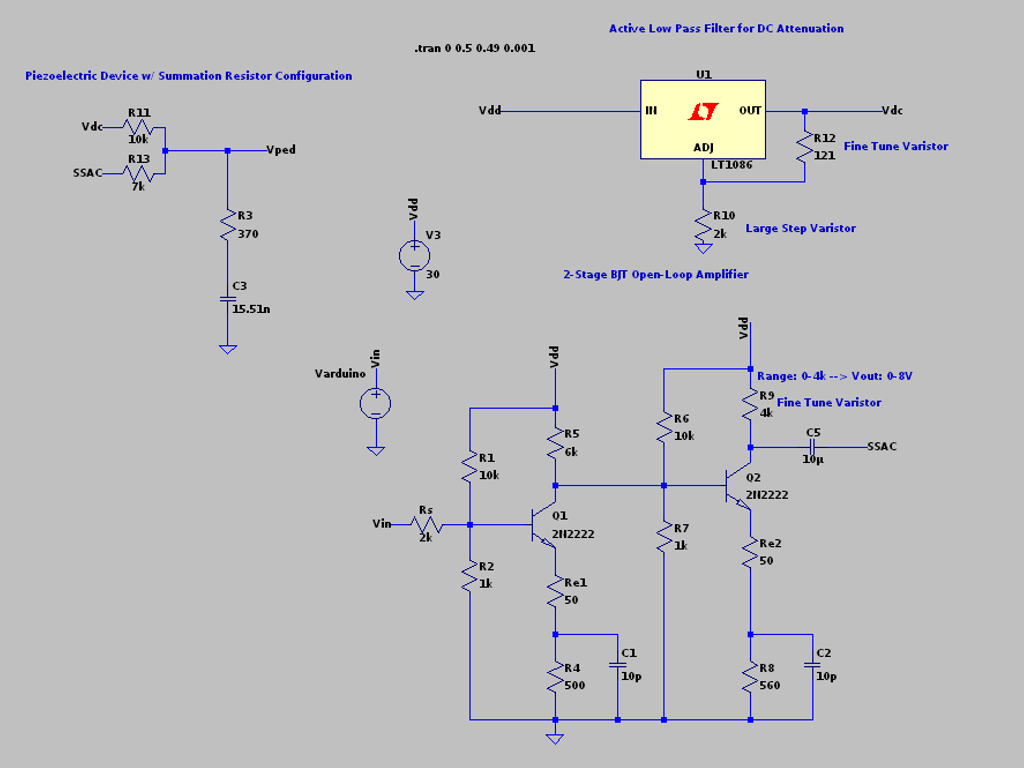
\includegraphics[width=\textwidth]{schematic_layout.png}
\caption{Schematic Layout Design}
\label{fig:schm}
\end{figure}

The following output was obtained by running simulations and changing the following values for each consecutive run (see Table~\ref{table1}). The following images correspond to the table values.

\begin{table}[!htpb]
\begin{center}
\begin{tabular}{*2c}
\toprule 
  \multicolumn{2}{c}{\textbf{\textit{Resistor Values for Specific Signal Output Specifications}}} \\ 
  \midrule
  \multicolumn{2}{c}{Maximum AC Signal and Maximum DC offset}\\ 
  \midrule
  \textbf{Resistor} & \textbf{Value} \\  
  
  $R_9$ & $4k\;\Omega$\\  
  
  $R_{10}$ & $5k\;\Omega$\\  
  \midrule
  \multicolumn{2}{c}{Maximum AC Signal and Minimum DC offset}\\ 
  \midrule
  \textbf{Resistor} & \textbf{Value} \\  
  
  $R_9$ & $4k\;\Omega$\\  
  
  $R_{10}$ & $100\;\Omega$\\  
  \midrule
  \multicolumn{2}{c}{Minimum AC Signal and Maximum DC offset}\\ 
  \midrule
  \textbf{Resistor} & \textbf{Value} \\  
  
  $R_9$ & $100\;\Omega$\\ 
  
  $R_{10}$ & $5k\;\Omega$\\ 
  \midrule
  \multicolumn{2}{c}{Minimum AC Signal and Minimum DC offset}\\ 
  \midrule
  \textbf{Resistor} & \textbf{Value} \\  
  
  $R_9$ & $100\;\Omega$\\  
  
  $R_{10}$ & $0\;\Omega$\\   
  \bottomrule
\end{tabular}
\caption{Resistor Values for Specific Signal Outputs}
\label{table1}
\end{center}
\end{table}

\begin{figure}[h!]
\centering
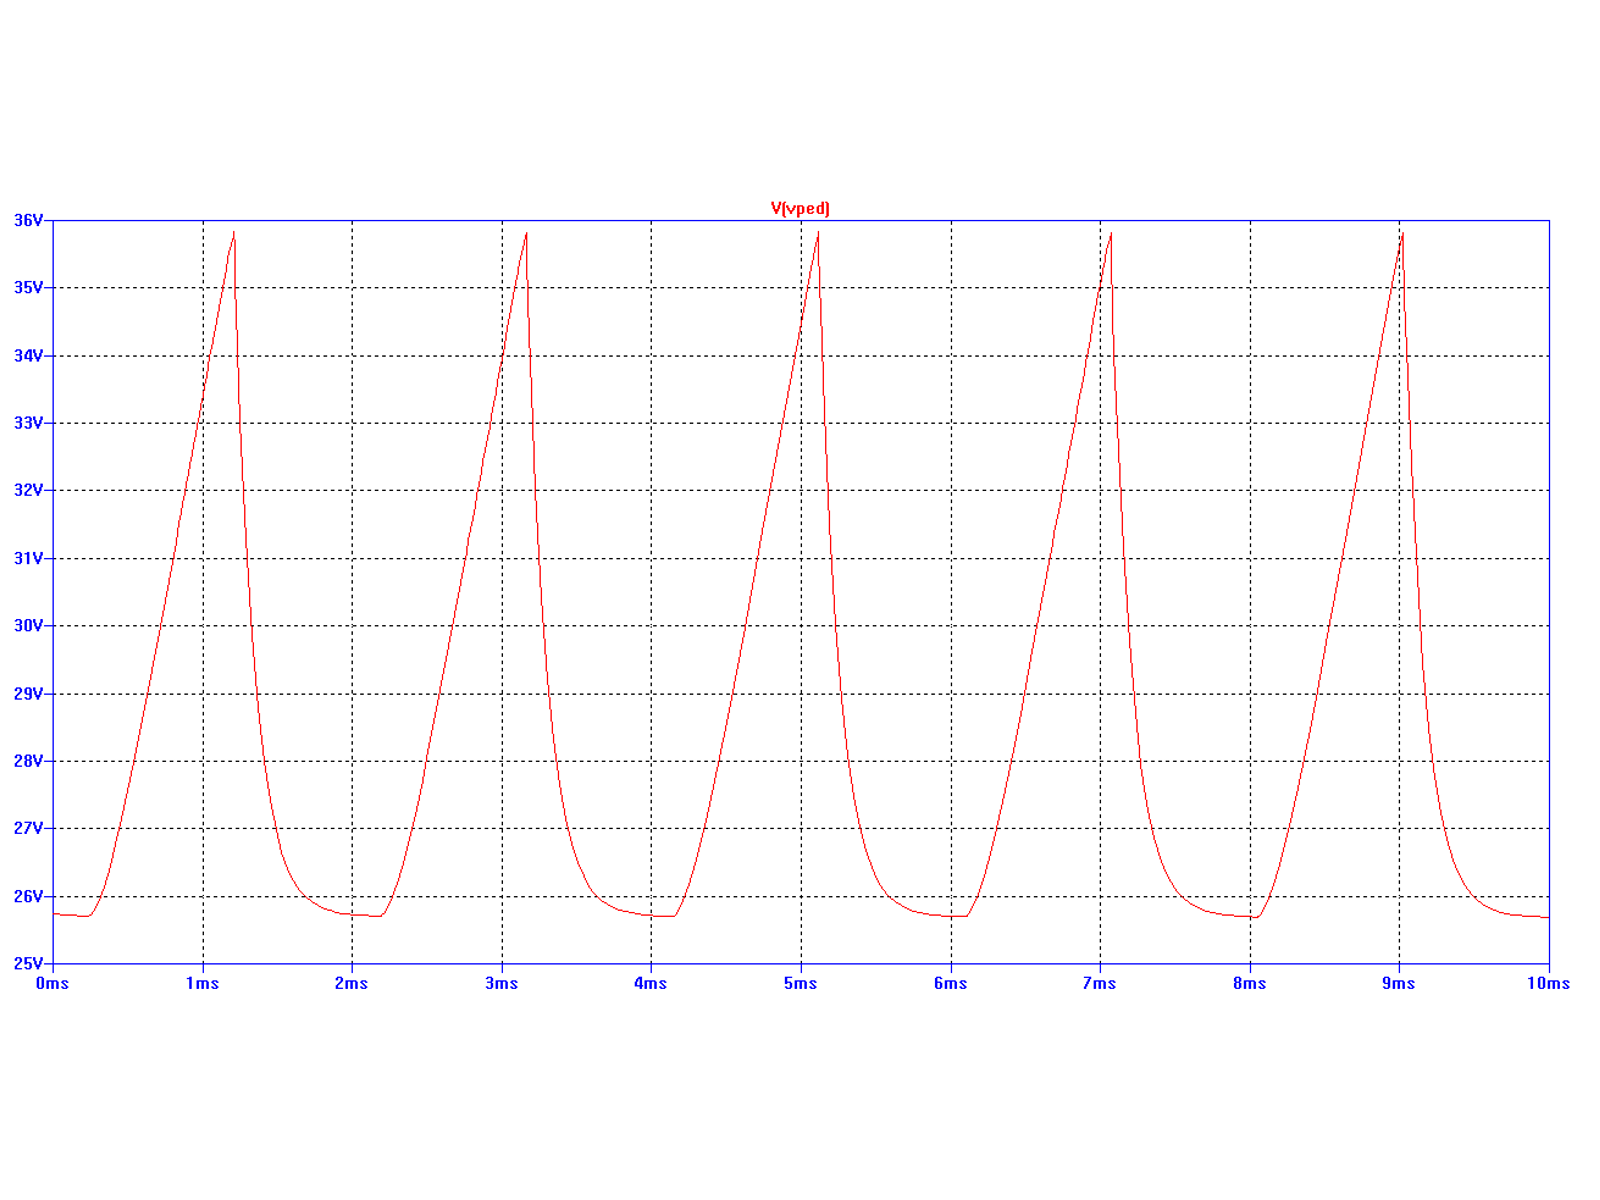
\includegraphics[width=\textwidth]{max_ssac_amp_dc.png}
\caption{Maximum AC Signal and Maximum DC offset}
\label{fig:maxmax}
\end{figure}

\begin{figure}[h!]
\centering
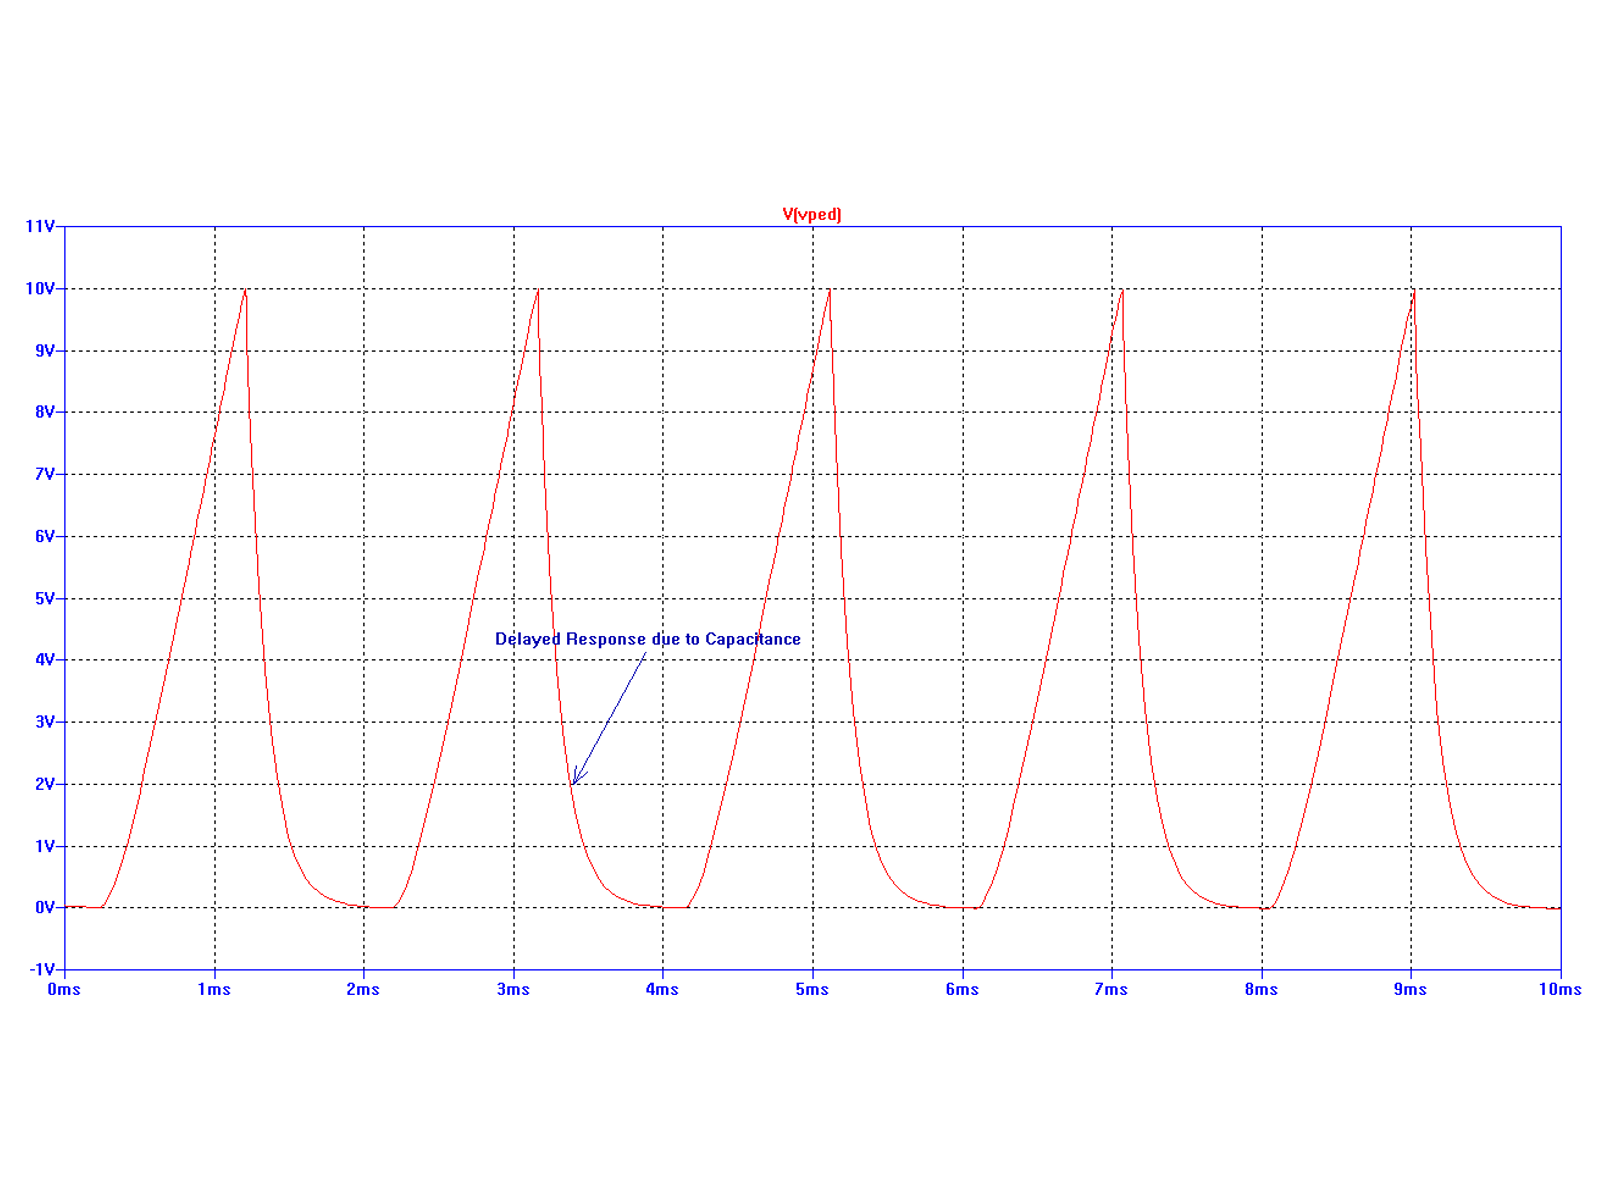
\includegraphics[width=\textwidth]{max_ssac_amp_no_dc.png}
\caption{Maximum AC Signal and Minimum DC offset}
\label{fig:maxmin}
\end{figure}

\begin{figure}[h!]
\centering
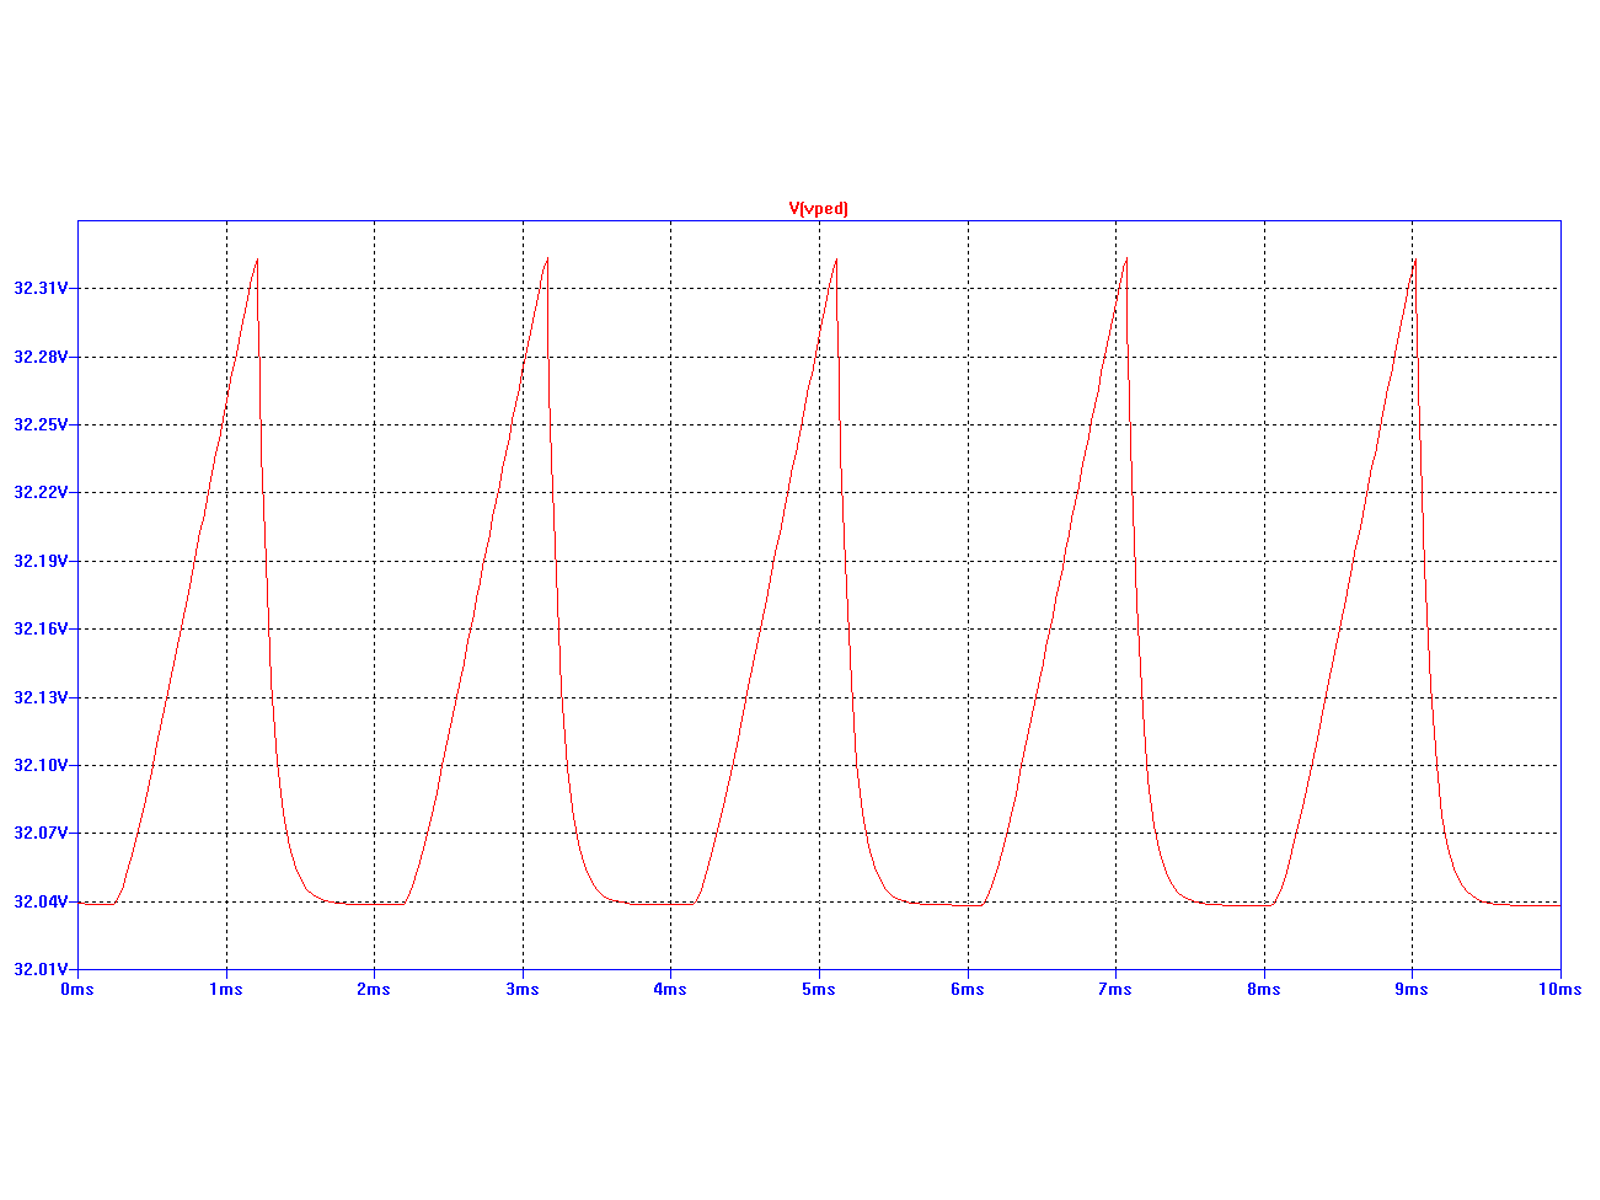
\includegraphics[width=\textwidth]{min_ssac_amp_dc.png}
\caption{Minimum AC Signal and Maximum DC offset}
\label{fig:minmax}
\end{figure}

\begin{figure}[h!]
\centering
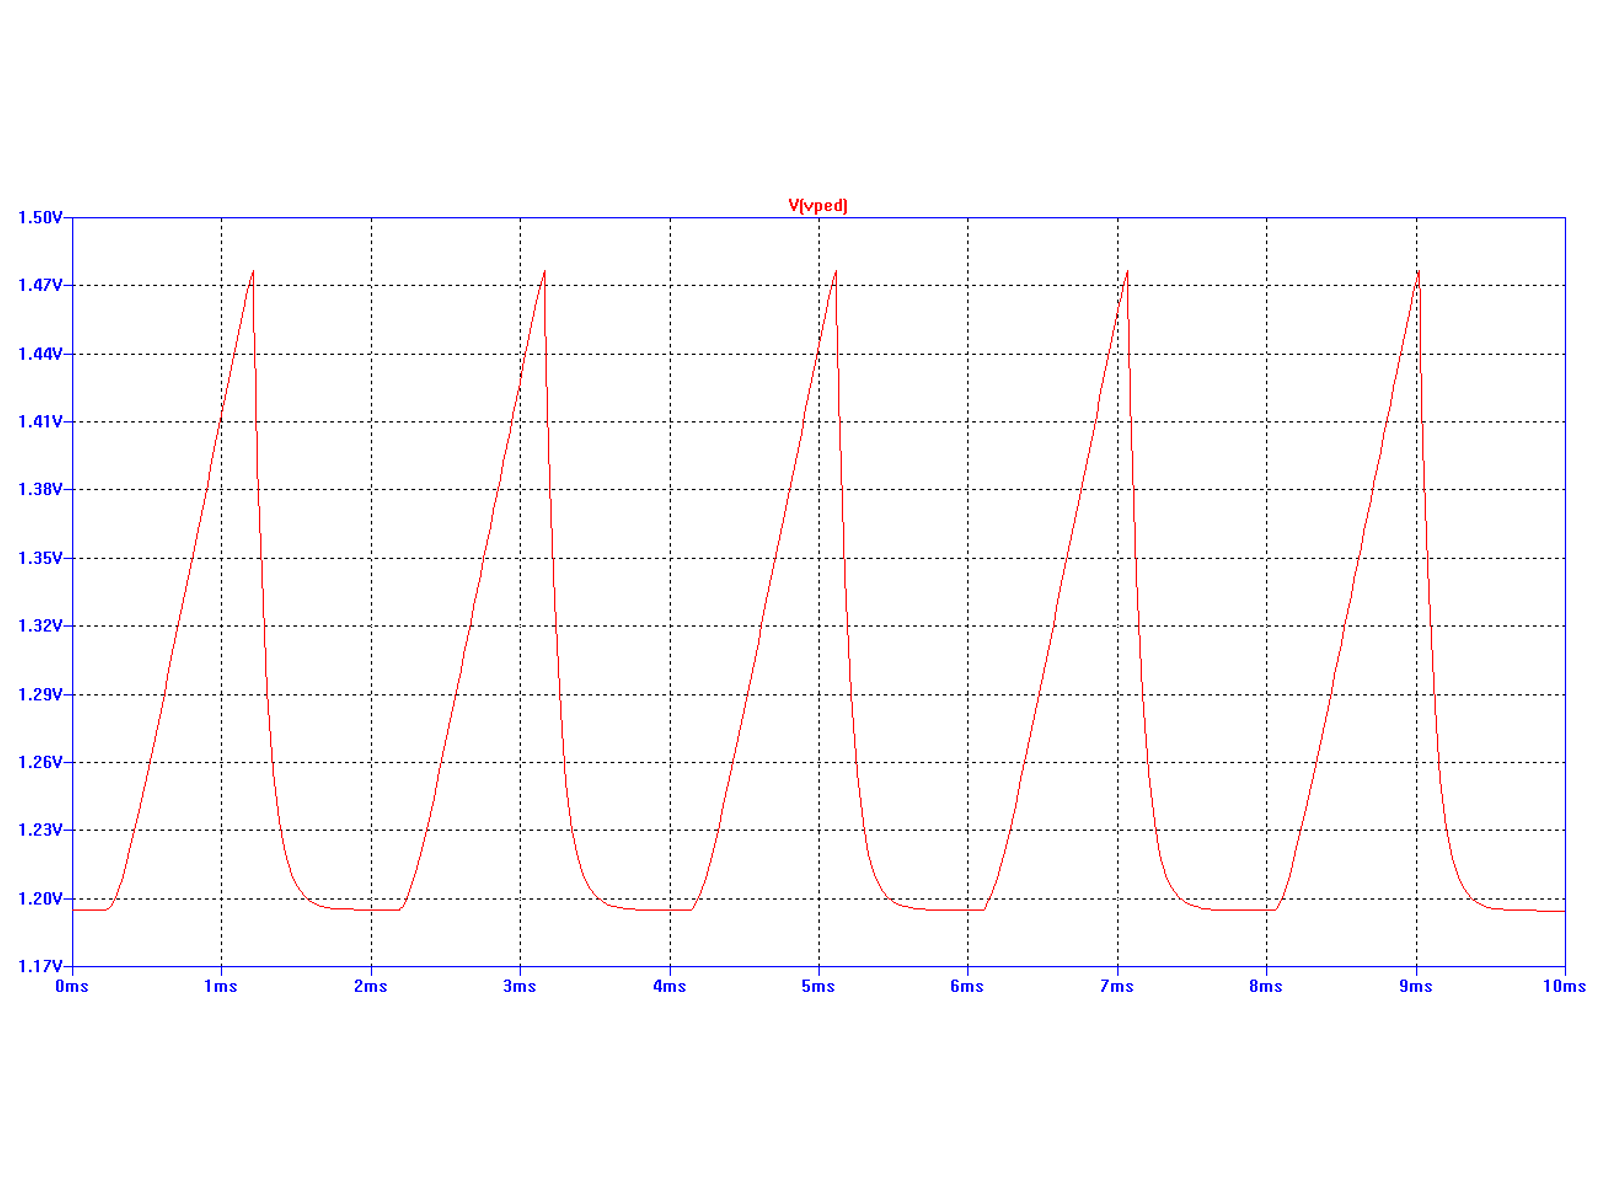
\includegraphics[width=\textwidth]{min_ssac_amp_no_dc.png}
\caption{Minimum AC Signal and Minimum DC offset}
\label{fig:minmin}
\end{figure}

\section{Conclusion}
Live circuit testing will be the next phase in the process. Most of this has already been done and proven, however, newer modifications may prove different results with new challenges that will need to be overcome. Overlooking this model the only issue I see is the variable DC voltage regulator I am using only allows for a minimum of 1.2 V when the AC signal is at its minimum. This issues severity will be determined in future tests.




\end{document}


